\chapter{Heterogeneous Knowledge Graph Construction}
\label{chap:kg}

\section{Motivation: Why a Heterogeneous Graph?}
\label{sec:kg_motivation}

The cleaned case JSONs produced by Chapter~\ref{chap:pipeline} are
already richer than the raw PDFs: each record carries typed entities,
rhetorical-role-segmented text, and an outcome label. The next question
is how to represent that richness in a way that a learner can actually
exploit.

A purely \emph{flat} representation -- concatenate the preamble, facts,
and arguments of a case, feed the blob into a transformer, and
classify -- has two costs. The first is that it throws away the typed
structure already present in the data: a court, a statute, a provision,
and a party are four different kinds of object with four different
kinds of evidential value for the outcome, and flattening them into one
token stream makes the model re-learn that from scratch. The second,
more important cost is that a flat representation has no way to
exchange information \emph{between} cases that share legally meaningful
objects. When Case~A and Case~B both cite IPC~498A, the flat view sees
the string twice; the graph view sees two cases attached to the same
\textsc{Statute} node and can, through one round of message passing,
let A's representation influence B's.

A heterogeneous graph captures both properties. It is
\emph{heterogeneous} because different node types carry different
features and different relational semantics (a \textsc{Court} is not a
\textsc{Lawyer} and they should not share a projection matrix), and it
is a \emph{graph} because the legally important relationships are
relational: a case \emph{is heard in} a court, an argument block
\emph{cites} a statute, a provision \emph{belongs to} a statute, a
lawyer \emph{argues in} an argument block. These are exactly the edges
a Graph Neural Network needs in order to reason about, rather than
merely classify over, the textual content.

The rest of this chapter describes the schema that implements that
intuition, the leakage-prevention strategy that keeps the schema from
accidentally leaking the outcome, and the text-embedding and scalar
features attached to each node.

\section{Graph Schema}
\label{sec:graph_schema}

The graph is constructed as a \textbf{full-star global graph}: every
case is a local "star" of text and entity nodes anchored on a
\textsc{Case} node, and a selected set of entity types are
\emph{shared} across cases so that stars of different cases are
stitched into one connected component.

\subsection{Node Types}

The reasoning-focused graph keeps \textbf{17 node types} in three
categories:

\begin{itemize}
  \item \textbf{The case node.} A single \textsc{Case} node per case,
    whose attributes store the outcome label, bucket, filing and
    decision dates (used for temporal gating), and bookkeeping
    metadata.
  \item \textbf{Text nodes.} Six types -- \textsc{Preamble},
    \textsc{Facts}, \textsc{Arguments},
    \textsc{Petitioner\_Arguments}, \textsc{Respondent\_Arguments},
    and \textsc{Other\_Lawyer\_Arguments} -- each carrying a
    \texttt{bge-m3} text embedding of the cleaned, leakage-filtered
    span they represent (Section~\ref{sec:text_features}).
  \item \textbf{Entity nodes.} Ten types: \textsc{Petitioner},
    \textsc{Respondent}, \textsc{Petitioner\_Lawyer},
    \textsc{Defence\_Lawyer}, \textsc{Lawyer}, \textsc{Court},
    \textsc{Judge}, \textsc{Statute}, \textsc{Provision}, and
    \textsc{Precedent}.
\end{itemize}

Four auxiliary NER types that OpenNyAI produces -- \textsc{Org},
\textsc{GPE}, \textsc{Date}, and \textsc{Case\_Number} -- are
explicitly \emph{removed} from the reasoning-focused graph
(\texttt{FORBIDDEN\_NODE\_TYPES} in the updated graph policy). They
carry little predictive signal for the outcome and would otherwise
inflate the node count and, worse, introduce weak, noisy edges that
dilute message passing. Their removal is one of the key differences
between the reasoning-focused variant used in this thesis and the
original baseline schema.

\subsection{Cross-Case Sharing}

Whether two cases share a node, or each hold a private copy of one,
determines whether a GNN can use that node as a cross-case conduit.
The policy (\texttt{reasoning\_graph\_policy.py}) is deliberate:

\begin{itemize}
  \item \textbf{Shared across cases}: \textsc{Statute},
    \textsc{Provision}, and \textsc{Precedent}. These are the
    \emph{law itself} -- citing IPC~420 in one case and IPC~420 in
    another is meant to be the same object, and sharing the node is
    what lets the GNN propagate information along the citation.
  \item \textbf{Local to each case}: everything else, including
    \textsc{Court}, \textsc{Judge}, and all \textsc{Lawyer}
    variants. These are \emph{identity proxies}: if a particular
    judge or a particular bench has a historical win/loss bias,
    sharing the node would let the GNN recover that bias as a free
    shortcut to the outcome -- exactly the kind of spurious signal
    the experimental design in Chapter~\ref{chap:results} is built
    to prevent. Keeping them local makes the model reason about the
    law, not about the docket.
\end{itemize}

\subsection{Edge Types}

The schema defines a concrete set of typed edges. The core structural
edges are:

\begin{itemize}
  \item \texttt{case--has\_preamble/has\_facts/has\_arguments--*text*}:
    attach each text node to its case.
  \item \texttt{case--has\_petitioner\_arguments/has\_respondent\_arguments/has\_other\_lawyer\_arguments--*text*}:
    attach party-specific argument blocks.
  \item \texttt{case--has\_petitioner/has\_respondent--*party*},
    \texttt{case--heard\_in--court},
    \texttt{case--decided\_by\_bench--judge},
    \texttt{case--has\_petitioner\_lawyer/has\_defence\_lawyer/has\_lawyer--*counsel*}.
  \item \texttt{arguments--cites\_statute--statute},
    \texttt{arguments--cites\_provision--provision},
    \texttt{arguments--cites\_precedent--precedent}: the citation
    backbone, attached to the \textsc{Arguments} node rather than to
    the case so that the citation sits in its legal-discourse
    context.
  \item \texttt{provision--belongs\_to\_statute--statute}: stitches
    the provision hierarchy into the graph so that a citation to
    Section~482 is two hops from IPC, not disconnected from it.
  \item \texttt{petitioner\_lawyer--citation--petitioner\_arguments},
    \texttt{defence\_lawyer--citation--respondent\_arguments},
    \texttt{lawyer--citation--other\_lawyer\_arguments}: connect each
    counsel to the argument block they are responsible for.
  \item \texttt{petitioner--is\_party\_in\_arguments--petitioner\_arguments},
    \texttt{respondent--is\_party\_in\_arguments--respondent\_arguments}:
    tie parties to their own argument blocks.
\end{itemize}

All edges are added with their reverse counterparts
(\texttt{include\_reverse\_edges}), and the final graph is passed
through \texttt{torch\_geometric.to\_undirected} so that HGT's typed
message passing can flow in both directions.

\paragraph{Shortcut edges that are intentionally removed.}
An earlier version of the schema added edges that let entities bypass
the arguments node -- e.g.\
\texttt{statute--used\_in\_arguments--arguments},
\texttt{judge--presided\_arguments--arguments},
\texttt{petitioner/respondent--is\_party\_in\_arguments--arguments} (to
the \emph{shared}, un-partitioned \textsc{Arguments} node). The updated
policy \emph{forbids} these edges (\texttt{FORBIDDEN\_EDGE\_TYPES}).
Keeping them would have created short paths from identity proxies to
the case representation that contribute little reasoning value but a
lot of spurious correlation; the thesis uses the reasoning-focused
schema for exactly this reason.

\subsection{Attributes}

Every \textsc{Case} node carries a binary outcome label
(\texttt{+1}~win, \texttt{-1}~loss) plus its bucket membership and the
dates needed for temporal gating. Every text node carries the raw
text (for downstream inspection only; the model never sees it
directly) and the pre-computed embedding. Every entity node carries
its canonical name and the canonicalisation metadata needed to
reproduce the merge. Edges are attributed with their relation type,
which is what the HGT layers use to index their per-relation
parameters (Chapter~\ref{chap:results}).

{\color{blue}
\subsection{Visualizing the Graph Structure}
\label{sec:graph_visualizations}

To provide a concrete visual intuition of the graph schema described above, we present diagrams of a single case graph and a multi-case subgraph. 

Figure~\ref{fig:single_case_graph} illustrates the local ``star-graph'' structure surrounding a single \textsc{Case} node. The node serves as an anchor connected to its text components (e.g., Preamble, Facts, Arguments) and its identity entities (e.g., Court, Judge, Lawyers). From the Arguments node, further citation edges branch out to Statutes and Precedents. 

Importantly, these outward citation edges maintain a strict chronological hierarchy: a newer case will only form a citation edge to a Precedent if $\text{precedent\_year} < \text{case\_year}$, and to a Statute if $\text{statute\_year} \leq \text{case\_year}$. This temporally-directed structure explicitly ensures that older cases cannot structurally link forward in time to newer artifacts.

\begin{figure}[htbp]
    \centering
    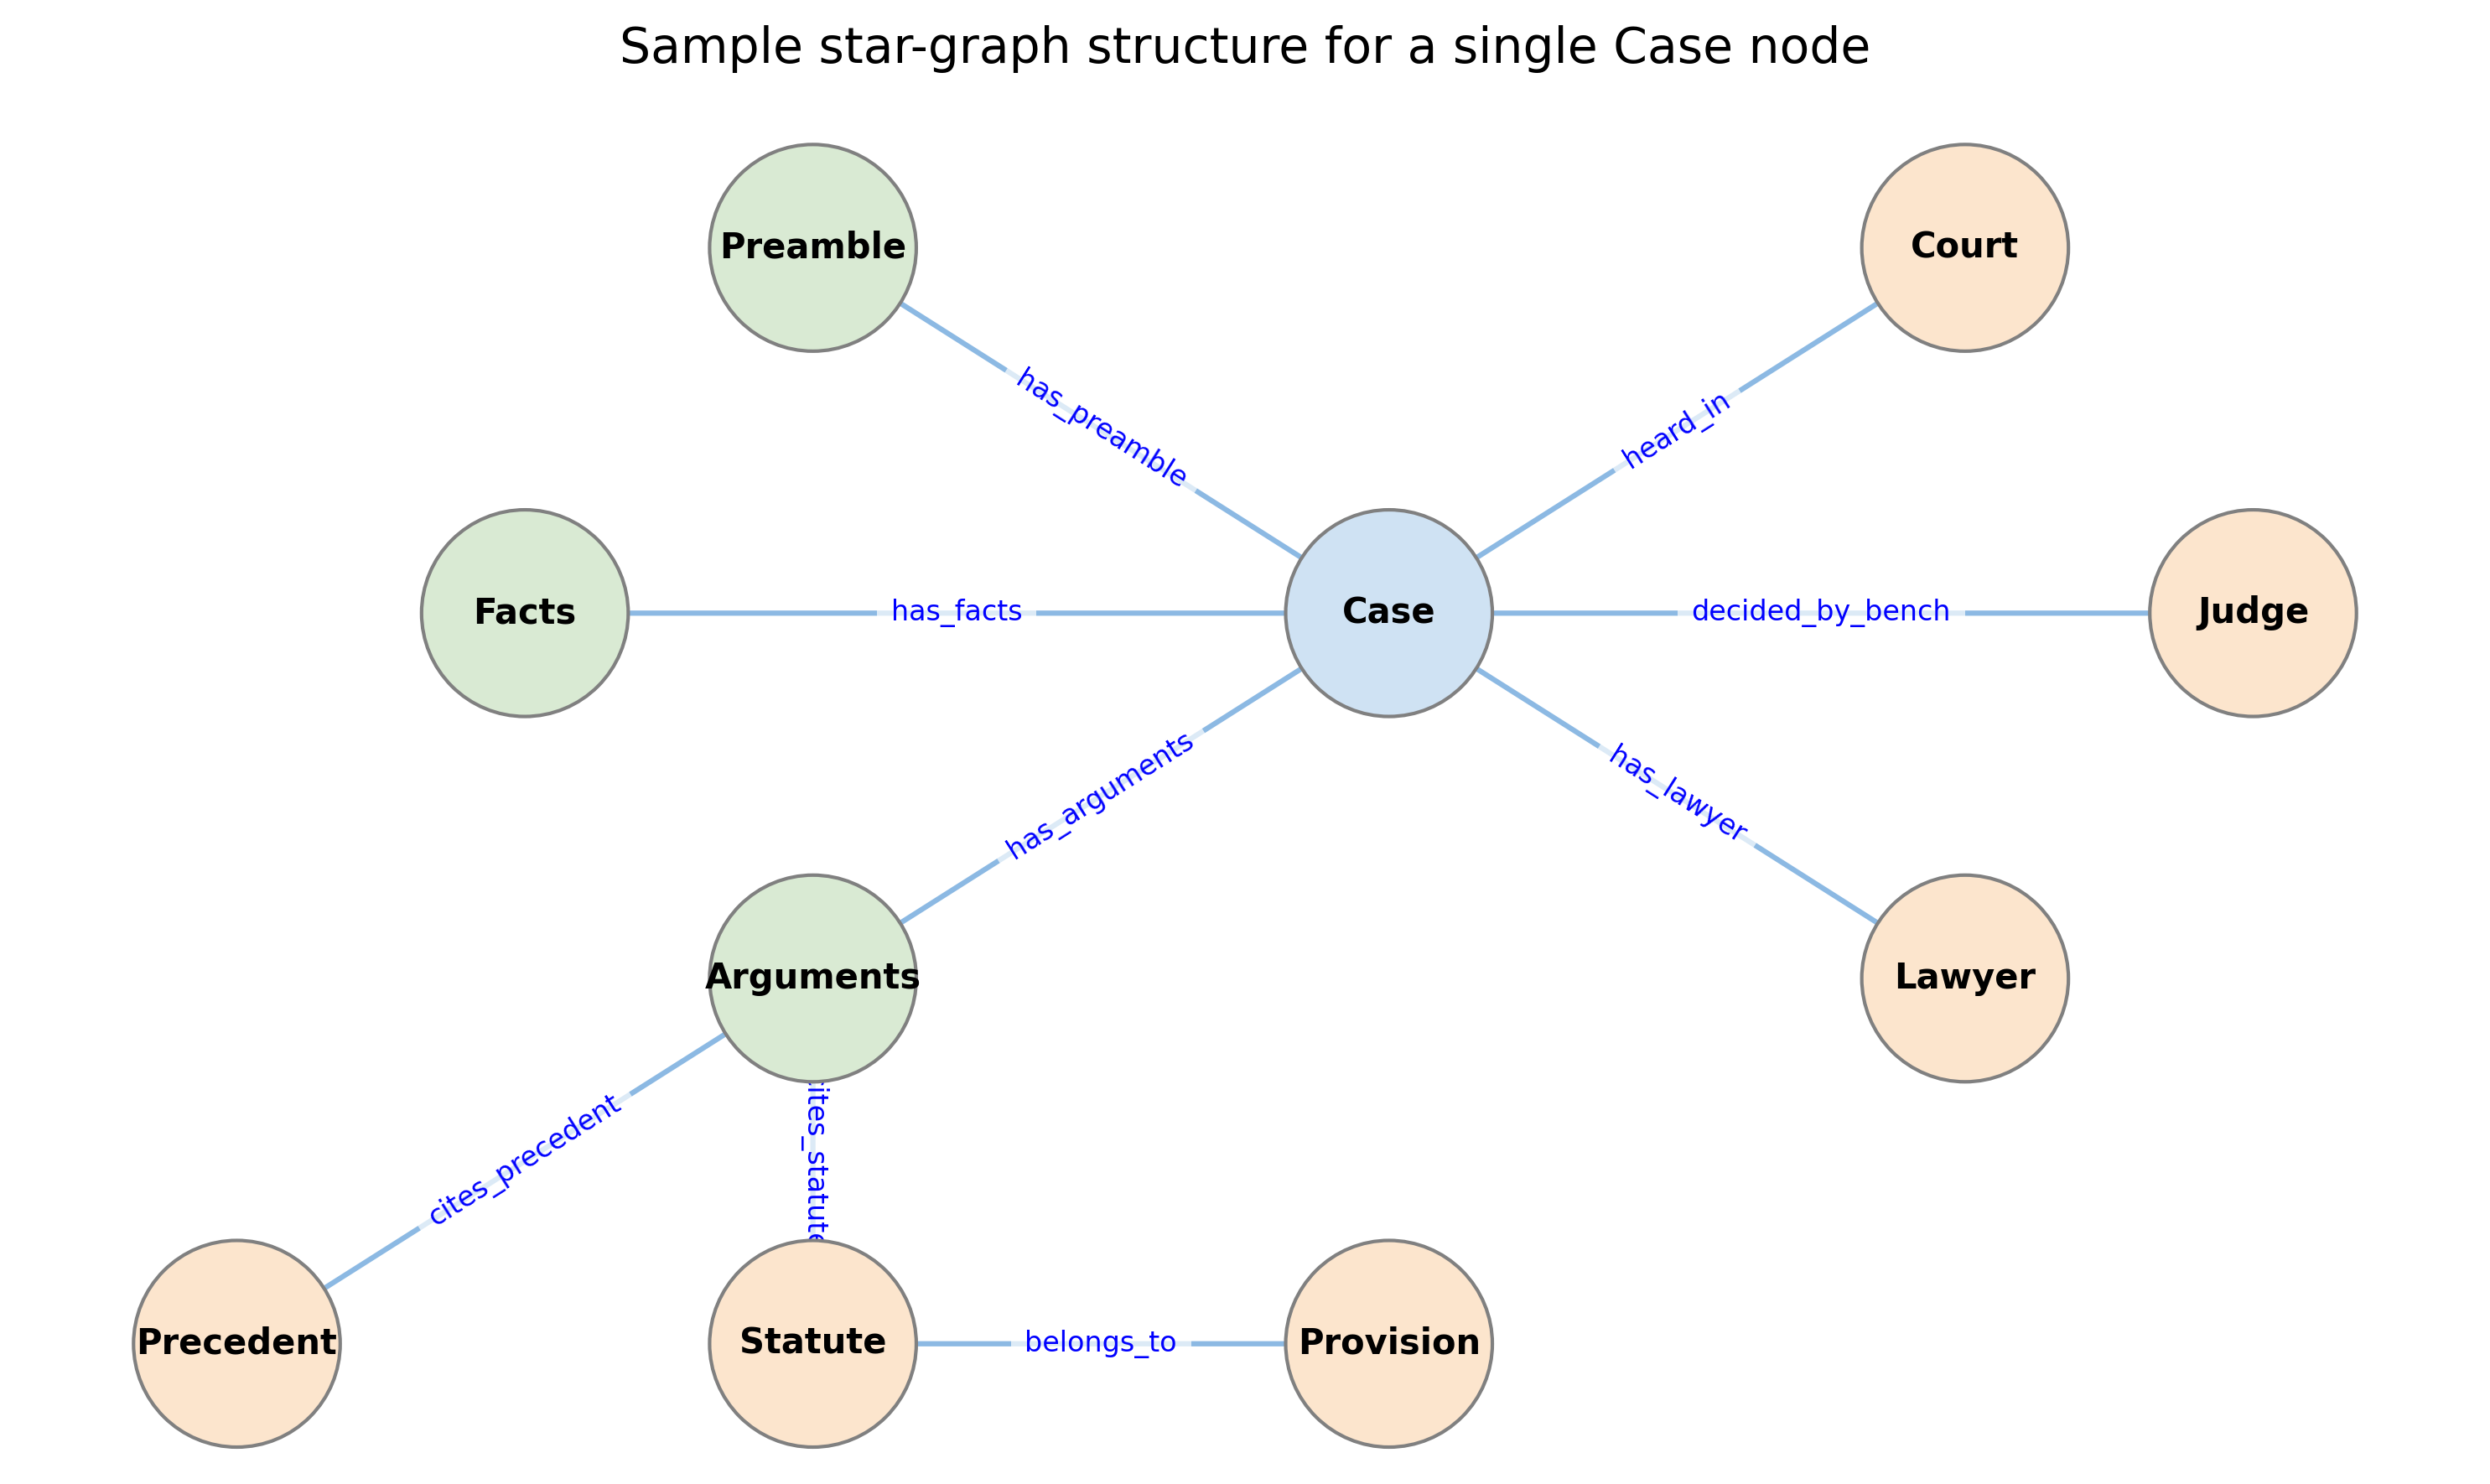
\includegraphics[width=\textwidth]{figures/single_case_graph.png}
    \caption{\textcolor{blue}{Sample star-graph structure for a single Case node. Various text blocks feature as text nodes, while details like Court and Judge form local entity nodes. The Arguments node branches out to cite shared legal concepts like Statutes and Precedents.}}
    \label{fig:single_case_graph}
\end{figure}

Figure~\ref{fig:cross_case_graph} demonstrates the cross-case sharing mechanism. To prevent spurious correlation (docket bias leakage), nodes like Courts and Judges are kept private to each case. In contrast, legal entities such as Statutes, Provisions, and Precedents are shared across cases, forming the cross-case conduits that allow the GNN to perform structural and legal reasoning without directly observing the outcome proxy.

\begin{figure}[htbp]
    \centering
    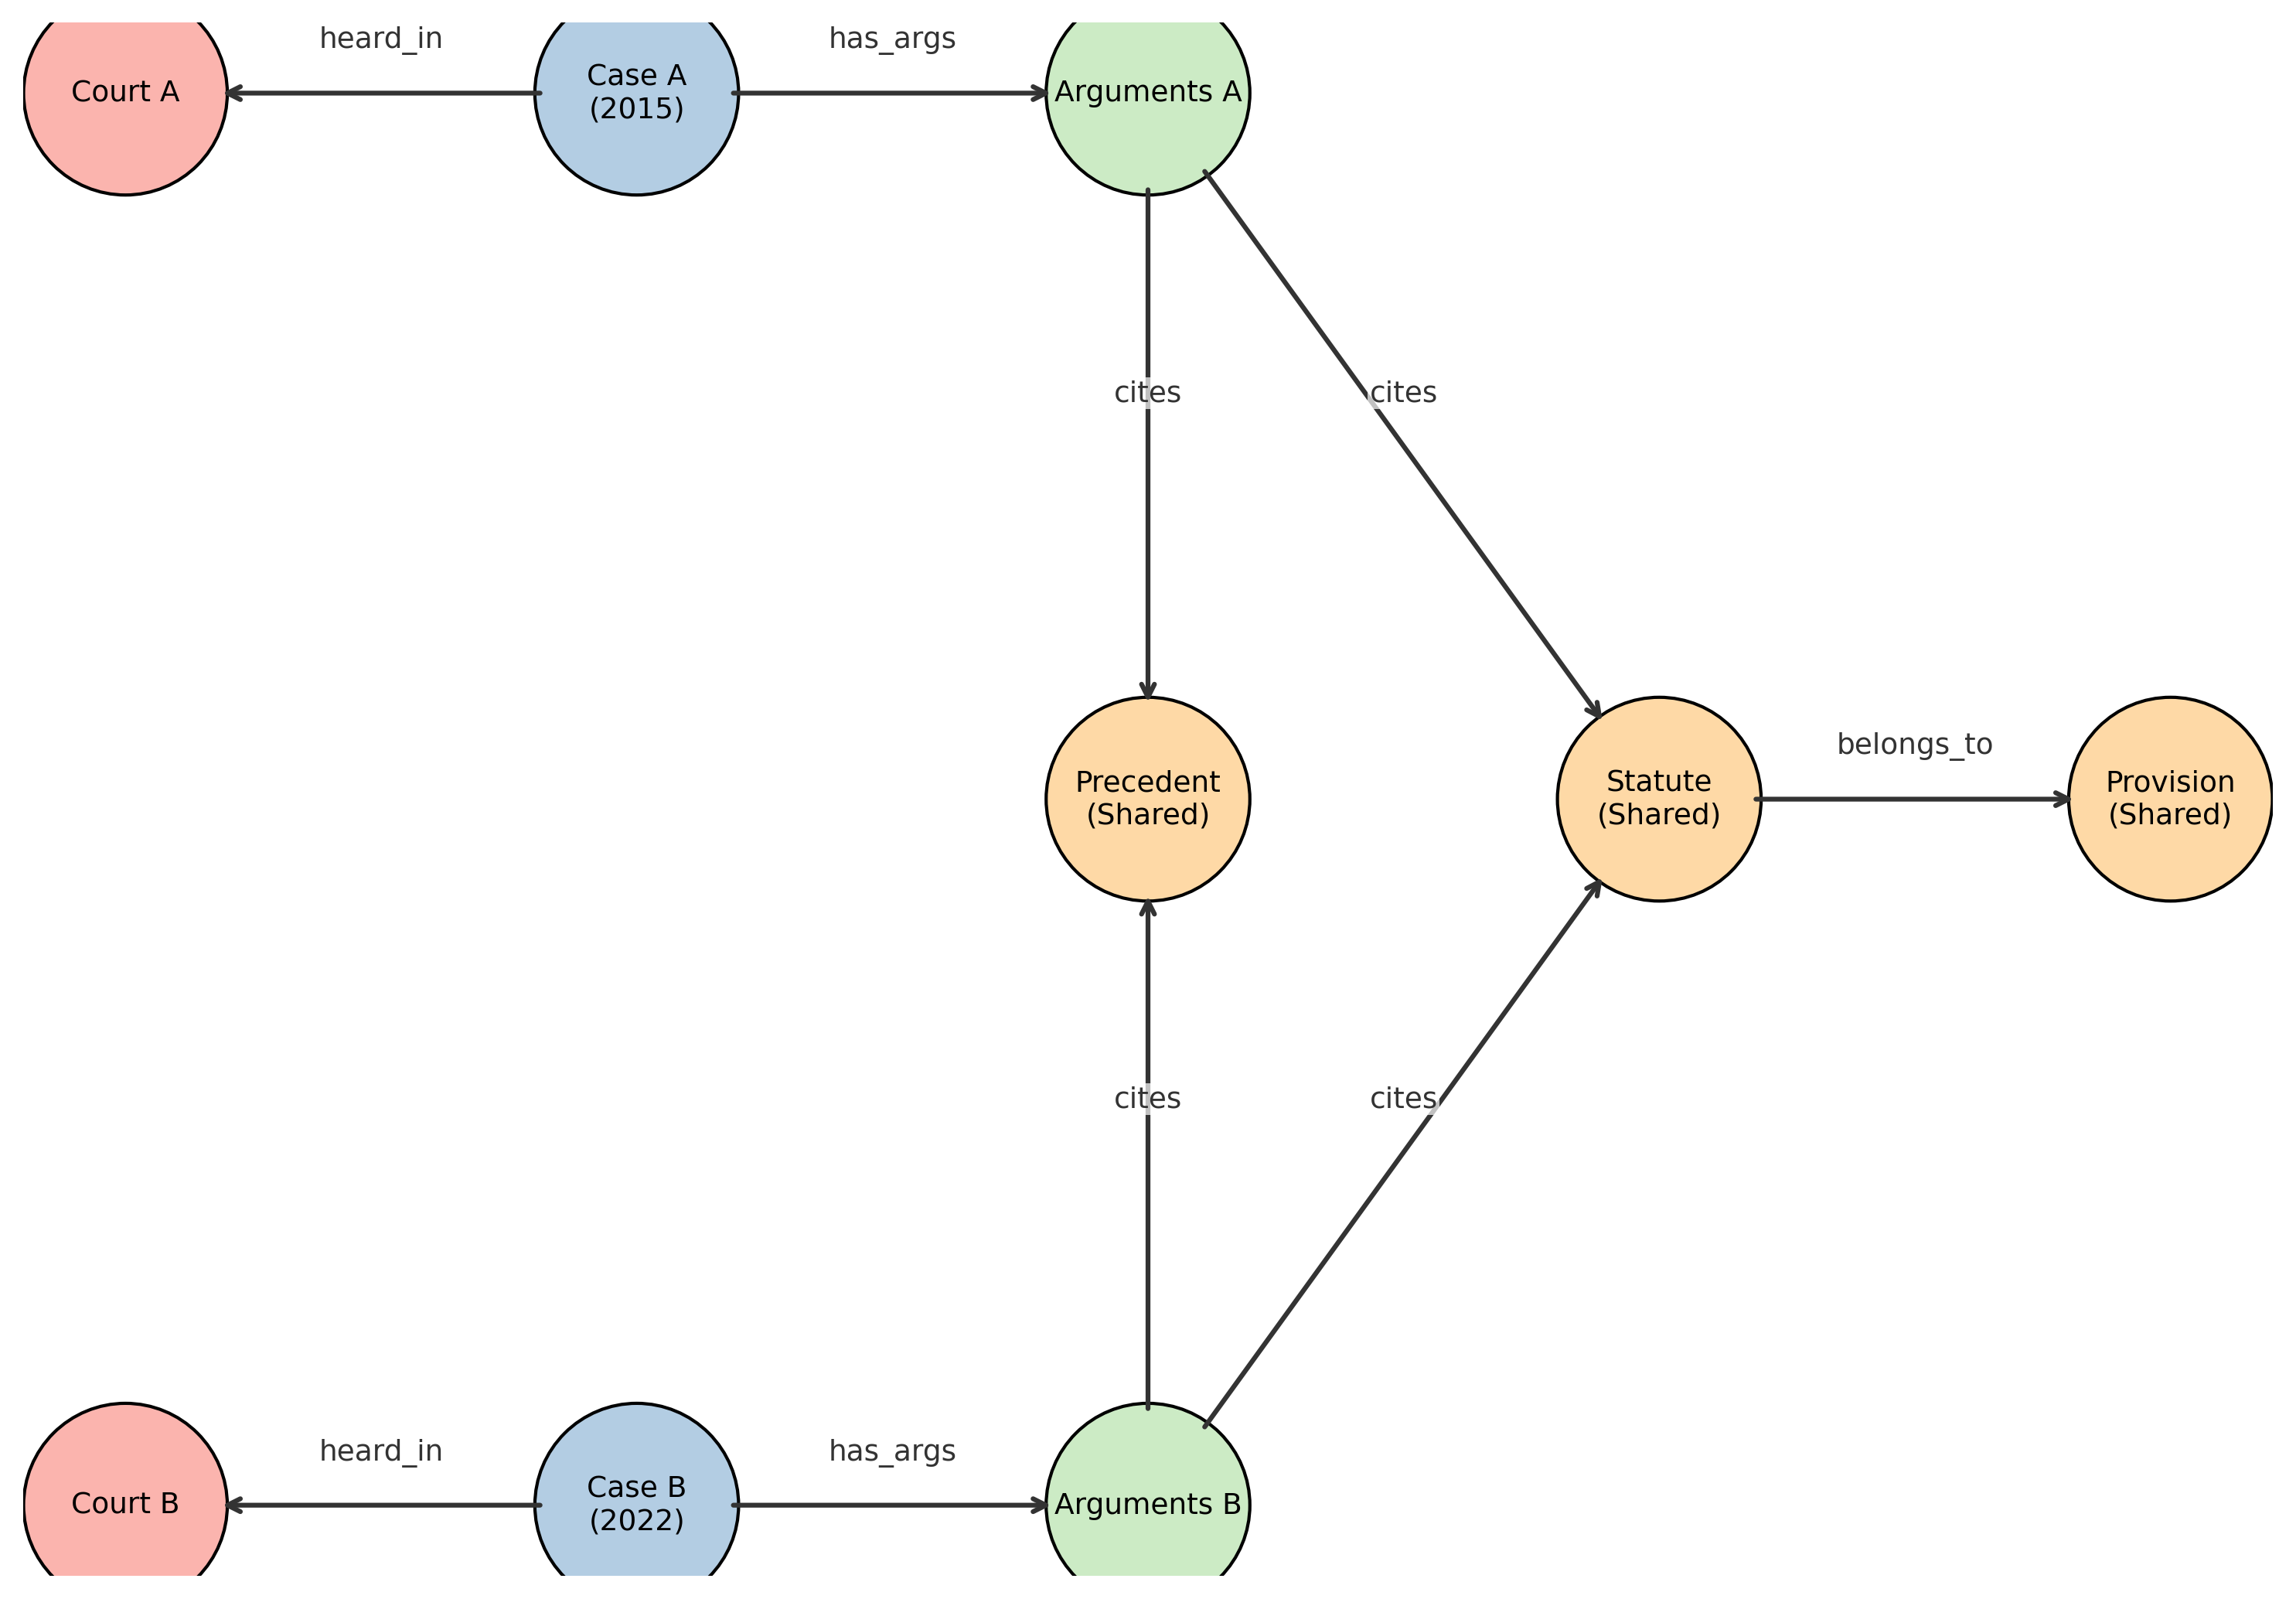
\includegraphics[width=\textwidth]{figures/schema_cross_case.png}
    \caption{\textcolor{blue}{Cross-connection of cases via shared nodes. Each case maintains its own local representations for identity entities to prevent shortcut leakage. Shared nodes like Statutes and Precedents act as legally-sound cross-case conduits for message passing.}}
    \label{fig:cross_case_graph}
\end{figure}
}

\section{Leakage Prevention Strategy}
\label{sec:leakage_prevention}

Legal judgment prediction has a notorious failure mode: models that
appear to predict the outcome are actually \emph{reading} it. The
construction pipeline defends against this at three distinct points.

\paragraph{1. Field-level removal.} The cleaning stage drops a fixed
set of \texttt{FORBIDDEN\_TOP\_LEVEL\_FIELDS} from the case JSON
before any graph is built:
\texttt{case\_outcome\_label},
\texttt{case\_outcome\_score},
\texttt{llm\_case\_outcome},
\texttt{decision\_text},
\texttt{rpc\_texts},
\texttt{short\_explanation}, and
\texttt{raw\_model\_response}. It also drops any
\texttt{raw\_result.summary.decision} block produced by the OpenNyAI
summariser.

\paragraph{2. Rhetorical-role filtering.} The
\texttt{FORBIDDEN\_ANNOTATION\_LABELS} set
(\{\textsc{RPC}, \textsc{RLC}\}) plus a label-string blacklist
(\texttt{decision}, \texttt{disposition}, \texttt{operative},
\texttt{order}, \texttt{rpc}) causes any annotation in those classes
to be removed from the summary before the text nodes are built.
Because \textsc{RPC} is where the court actually pronounces the
result, this is the single most important filter: without it, the
\textsc{Arguments} text node would contain the verdict verbatim.

\paragraph{3. Phrase-level masking.} A list of
\texttt{DEFAULT\_LEAKAGE\_PHRASES} --
\emph{``petition stands disposed of''},
\emph{``appeal is allowed''},
\emph{``set aside''},
\emph{``quashed''}, and so on -- is compiled into case-insensitive,
whitespace-tolerant regex patterns and applied as a sub-sentence
scrubber across every retained text field. Every match is logged in a
per-case \texttt{leakage\_audit}, and the phrase itself is replaced
with a \texttt{[LEAKAGE\_MASK]} token. This catches residual
decision-bearing fragments that the RR filter missed because they were
embedded inside a \textsc{Facts} or \textsc{Arguments} sentence rather
than tagged as \textsc{RPC}.

\paragraph{4. Temporal gating on shared entities.} Sharing a
\textsc{Precedent} or \textsc{Statute} node across cases would leak
future information if a precedent decided in 2022 were attached to a
case from 2015. The graph builder therefore enforces a temporal rule
inside \texttt{case\_star\_builder}: a precedent citation edge is added
only when $\text{precedent\_year} < \text{case\_year}$, and a statute
citation edge only when $\text{statute\_year} \leq \text{case\_year}$.
This keeps the cross-case conduit legally honest.

\paragraph{5. Audit trail.} Every case carries a \texttt{leakage\_audit}
structure recording the fields dropped, the annotations removed, the
decision text removed, and every phrase-level mask. The audit is kept
with the graph cache so that any future claim of leakage can be
\emph{disproved}, not merely argued against.

The combined effect of these five gates is that the text a GNN layer
eventually sees through its text-node features is a pre-decision
representation of the dispute -- who the parties are, what happened,
what each side argued, and what law they cited -- with the decision
itself systematically withheld.

\section{Text Embedding and Feature Extraction}
\label{sec:text_features}

\subsection{The \texttt{bge-m3} Text Encoder}

All text nodes are featurised with \texttt{BAAI/bge-m3}, a multilingual
sentence-transformer with a $1024$-dimensional output, run through the
\texttt{sentence\_transformers} library. The choice of \texttt{bge-m3}
is driven by two concrete requirements: (i) Indian legal text mixes
English with Hindi and regional-language transliterations, Latin-script
legal abbreviations, and citation fragments, and \texttt{bge-m3}'s
multilingual training data handles this noticeably better than
English-only encoders; and (ii) the model is strong in retrieval
settings, which aligns with the graph's use of embeddings as
comparison features across cases.

\paragraph{Configuration.} The encoder is run with
\texttt{batch\_size=16}, \texttt{max\_length=512}, on GPU, and with
multi-process mode enabled. When multiple CUDA devices are visible the
encoder spins up one worker per device, distributes the text list, and
merges the results, which is what makes encoding millions of argument
and facts spans tractable in wall-clock terms.

\paragraph{Hierarchical chunking for long spans.} Legal judgment
\emph{Facts} and \emph{Arguments} sections routinely exceed the
model's $512$-token window. For texts longer than the configured
character limit, the encoder splits them into overlapping,
sentence-boundary-aligned chunks, encodes each chunk independently,
and mean-pools the resulting vectors. This preserves a consistent
$1024$-dimensional representation per text node regardless of input
length, while avoiding the information loss of a hard truncation.

\paragraph{Caching.} Embeddings are cached per namespace with a
deterministic hash of the input ids, texts, and encoder configuration.
Re-running the graph build with an unchanged encoder loads cached
vectors in seconds; changing any encoder-sensitive field
(\texttt{backend}, \texttt{model\_name}, \texttt{max\_length},
\texttt{hierarchical\_chunk\_chars}) invalidates the cache. A
\texttt{hashing} fallback encoder is available for local debugging
when GPU resources are unavailable.

\subsection{Node Feature Assembly}

For each node type the final per-node feature vector is the
concatenation of:

\begin{itemize}
  \item the $1024$-dim \texttt{bge-m3} embedding of the node's canonical
    text (for text nodes, that is the full span; for entity nodes,
    that is the canonical name);
  \item scalar node-level features: local frequency in the case,
    section-of-first-mention indicators (\texttt{seen\_in\_preamble},
    \texttt{seen_in\_arguments}), type one-hot, and for shared entity
    types the log global frequency across the corpus;
  \item for the \textsc{Case} node, bucket one-hot and the outcome
    label is attached only as the supervision target, never as a
    feature.
\end{itemize}

Because different node types carry different feature dimensionalities,
the HGT model used in Chapter~\ref{chap:results} begins with a
per-node-type linear projection (\texttt{input\_projections}) that maps
all features into a common hidden dimension before the first
heterogeneous message-passing layer. This is the mechanism that lets
the graph remain genuinely heterogeneous at the feature level while
still admitting a uniform message-passing computation.
